\chapter{Adaptive Learning}
\label{chap:adaptive-learning}

% TODO:
% - incorporate other notes from my/thesis gdoc
% - inspiration from relevant articles
% - add references for provided examples (playing chess, autonomous car, ...)

From playing chess to driving an autonomous car,
  artificial intelligence proved to be a mighty tool
  for tackling difficult algorithmic tasks.
The power of artificial intelligence can be also used
  to develop a personalized adaptive system for learning programming.
Such system would create an optimal learning experience for each student
  by providing them with problems of difficulty matching their skill,
  so that the student stays challenged and interested in solving them.

In the existing systems (\ref{sec:existing-systems}),
  the sequence of tasks is the same for everybody.
As a result, the progress is necessarily too slow for some students,
  who could skip some of the tasks,
  while being too fast for others,
  who could highly benefit from solving a couple of other similar tasks.
Artificial intelligence can be used to personalize
  the sequence of tasks for every student.
By giving the student a suitable task
  -- neither too easy, nor too difficult --
  it can help the student to get into the state of flow
  (\ref{sec:motivation.challenge}).

In addition to choosing the most suitable task for given student,
  artificial intelligence has also other possible uses in learning systems,
  for example automatic hints generation \cite{generating-hints}
  or skills visualization (TBA: ref).
Furthermore, artificial intelligence techniques can be used
  to analyze collected data offline.
Such analyses can reveal problematic tasks,
  or suggest how to group tasks into categories (TBA: ref).

Adaptive learning systems have been already successful in some domains.
For instance, Map Outlines%
  \footnote{Available at \url{https://outlinemaps.org}.},
  developed by Adaptive Learning research group at Masaryk University,
  is an intelligent web application for learning geography.
It has been used by tens of thousands of students
  and online experiments have confirmed
  that the adaptivity of the system helps to improve the learning outcome
  \cite{alg.evaluation-geography}.
In addition to geography, similar adaptive web applications
  for learning anatomy%
  \footnote{Available at \url{https://practiceanatomy.com}.},
  biology%
  \footnote{Available at \url{https://poznavackaprirody.cz} (in Czech only).},
  elementary mathematics%
  \footnote{Available at \url{https://matmat.cz} (in Czech only).},
  and Czech grammar%
  \footnote{Available at \url{https://umimecesky.cz} (in Czech only).},
  were developed by the research group in recent years.

Section \ref{sec:student-modeling} presents how to model students
  in the context of learning programming.
Sections \ref{sec:task-recommendation} and \ref{sec:mastery-learning}
  then describe how to use these models to make a learning system adaptive.
Finally, section \ref{sec:metrics-and-evaluation} discusses how to evaluate
  different models or even whole learning systems.


\section{Student Modeling}
\label{sec:student-modeling}

For the system to be adaptive, models of
  a student skill, task difficulty, and student-task interaction
  need to be designed, implemented, and evaluated using collected data.
The purpose of these models is to predict the probability that a given student
  would solve a given task
  and also the time the student would need to complete the task.


\subsection{Data}
\label{sec:student-modeling.data}

To learn model parameters, such as difficulty of individual tasks, some data is needed.
What data and how much data is needed differs across models.
Some data about tasks are independent of students;
therefore, they can be obtained in advance,
which can be useful for initial task difficulties estimates.
Three types of task data are distinguished:

\begin{itemize}
  \item task statement (including name and world description),
  \item sample solution (or multiple solutions),
  \item expert labels (e.g. covered concepts).
\end{itemize}

Task statements are always available,
  because they are needed to present tasks to students.
However, obtaining sample solutions and expert labels
  incurs additional costs for a new system.
% TODO: Note that quite often, systems needs sample solutions and some labels
%       for the presentation purposes anyway.
Moreover, they can be noisy and imperfect.
For example, an annotator can forget to include some labels
  or even make a mistake in the sample solution.

Once the task is deployed in the running system,
  rich data can be collected from each interaction between a student and a task:
\begin{itemize}
  \item whether the task was eventually solved,
  \item solving time,
  \item number of clicks, number of code executions,
  \item program snapshots (e.g. after each code change),
  \item rating or labels provided by the student (e.g. perceived difficulty).
\end{itemize}

% TODO: also consider to include hints in the list
% TODO: mention different granularity levels for taking program snapshots (+cite)

\subsection{Item Response Theory}
\label{sec:irt}

The simplest version of item \emph{item response theory} (IRT)
  \cite{irt-visual-guide}
  models each student by a one-dimension skill $s$,
  and each task by a one-dimension difficulty $d$.
IRT assumes that the probability of a student with skill $s$
  successfully solving a task with difficulty $d$
  is given by the following function:
  \begin{equation}\label{eq:logistic}
  P(s, d) = \frac{1}{1 + e^{-(s - d)}}
  \end{equation}

% TODO: mention 2-parameter model (explain discrimination parameter)
\begin{figure}[h]
  \centering
  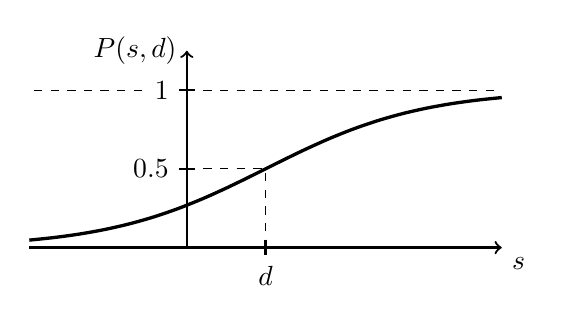
\begin{tikzpicture}[domain=-2:4, smooth, samples=20, scale=1]
  \draw [thick, ->] (-2,0) -- (4,0) node [below right] {$s$};
  \draw [thick, ->] (0,0) -- (0,2.5) node [left] {$P(s,d)$};
  \draw [thick] (-0.1,1) node [left] {$0.5$} -- (0.1,1);
  \draw [thick] (-0.1,2) node [left] {$1$} -- (0.1,2);
  \draw [thin, dashed] (0,2) -- (4,2);
  \draw [thin, dashed] (0,1) -- (1,1) -- (1, 0);
  \draw [thin, dashed] (-0.57,2) -- (-2,2);
  \draw [thick] (1,0.1) -- (1,-0.1) node [below] {$d$};
  \draw [very thick] plot (\x, {2 / (1 + exp(1 - \x))});
  \end{tikzpicture}
  \caption{One-parameter Unidimensional Logistic Model}
  \label{fig:logistic-model}
\end{figure}

This basic model was originally developed for a simple knowledge testing
  and therefore it assumes a single constant skill.
However, programming skill is multidimensional;
  for example, one student can be proficient with functions and struggle with loops,
  while another student can master loops and struggle with functions.
Furthermore, these skills should be ideally changing significantly during
  the interaction with the system, because students are learning.

Another drawback of the IRT is that it only uses
  the binary data about successes and failures.
As nearly all interactions in programming learning systems end with a solved task,
  it would be more useful to work with solving times,
  which can provide more information about students' skills.

Item response theory can be extended to overcome these limitations.
\emph{Problem Response Theory} (PRT)
\cite{alg.problem-response-theory, pelanek-student-modeling-times}
% TODO: only cite the more relevant paper (or extend this section and cite both
% on relevant places)
predicts problem solving times instead of probability of success,
assuming an exponential relationship between a problem solving skill
and the time to solve a problem.
PRT can be formulated to use multidimensional skills.
The model parameters (skills and difficulties) can can be estimated from the data
  using one of the \emph{maximum likelihood estimation} algorithms.
  % TODO: cite paper describing the parameters estimation (or MLE?)
% (for IRT, it's \cite{irt-theory-and-practice}, but PRT would be better)

% TODO: find and provide the details about the learning extension of PRT
% (isn't it already the elo?)

% TODO: Add note that the assumption of exponential relationship is justified
% by observed solving solving times distribution and it is also intuitively
  % plausible - multiplicative nature of solving times.



\subsection{Elo}
\label{sec:elo}

The Elo model \cite{alg.elo}
  extends the logistic model presented in section \ref{sec:irt}
  to capture changing knowledge.
Inspired by the rating of chess players \cite{elo-rating},
  the model interprets each attempt  to solve a task
  as a ``match'' between the student and the task.
After this match ends, skill and difficulty estimates are revised.

If the student solves the task faster than expected by the model,
  their skill is increased and the difficulty estimate of the solved task is decreased.
On the contrary, if the student fails to solve the task or if takes them too long,
  their skill is decreased and the difficulty estimate of this task is increased.

% TODO: formulas (for time-variant of elo)
% TODO: mention differnet updates for tasks (exponentially decayed) and
% students (their skill is assumed to change and not converge)

The main advantage of using the Elo model is its simplicity, flexibility,
  good performance and intrinsic online nature, which allows for immediate
  updates of parameters as students are interacting with the system.

% TODO: include other models, PFA, BKT etc.


\subsection{Concepts}

% TODO: consider to move this section before the description of individual
% models
% TODO: fix and mention used terminology: concept vs. skill

A vast amount of research in the field of adaptive learning
  restricts its attention to a one-dimensional skill.
This assumption is reasonable for many logic puzzles (e.g. sudoku);
however, solving programming tasks requires multiple diverse skills,
  such as loops, conditional commands, or functions.
It is possible to master loops while struggling with functions,
  and vice versa.

As mentioned in sections \ref{sec:irt} and \ref{sec:elo},
  both the IRT and Elo models can be extended to work with multidimensional skills.
% TODO: However, the way they compose multiple skills into a single prediction
% is not completely justified / can differ depending on domain/skills (e.g.
% adding skills vs taking best/worse)
Although modeling multiple skills seems useful,
  there is a trade-off between the complexity of the model (number of skills)
  and how well (or how fast) the parameters can be estimated.
More parameters require more data and time for the estimates to converge.
% TODO: which is especially concern for students; 1. predictions needed
% immediately for new students (no/little data), 2. students' skills are
% assumed to change (tasks didn't have these problems)


% \subsection{Learning Concepts from Data}

Concepts can be either defined manually or detected automatically
  \cite{niznan-thesis}.  % TODO: specify chapter/pages
Manually selected concepts, such as loops and conditional commands,
  have the advantage of being interpretable,
  so they can be used for skills visualizations in the user interface
  to provide students with the information about their learning progress.
Furthermore, no data needs to be collected in advance,
  while the automatic techniques require a lot of data to provide stable results.  % TODO: how much?


% \subsection{Prerequisites}
Undoubtedly, there are some relationships between skills;
  for example, nested loops cannot be mastered without mastering simple loops.
The hierarchical structure between concepts can be modeled
  as a directed acyclic graph (DAG),
  where each vertex is a concept and each edge represents a prerequisite.
Having DAG of concepts then allows to model students using Bayes networks
  \cite{its-programming}.

% TODO: simple diagram: DAG of concepts example

\section{Task Recommendation}
\label{sec:task-recommendation}

Student models are used by an \emph{instructional policy} to recommend
  the most suitable task for a student.
In spite of having all the predictions about success probabilities
  and time estimates available,
  task recommendation is not an easy task.
First, it is not clear what difficulty level is optimal.  % TODO: example (75 % of success etc.)
Second, it may vary for different students, domains or types of problems.
Furthermore, optimal difficulty is not the only criterion to be considered.
For instance, diversity of tasks is important to keep students interested.
No principled techniques for task recommendation have been developed yet;
however, several heuristic approaches have been used
  and proved to work well (TBA: ref).

Task recommendation is not a necessary requirement
  for the system to be adaptive.
Student models can be utilized by other means to achieve personalized behavior,
  e.g. in mastery learning (section \ref{sec:mastery-learning}).
The system can also just provide students with predicted solving times
  and let them to choose the next task they want to solve.

Showing predictions can be already perceived as a very mild form of recommendation.
Indeed, recommendations can range from \emph{soft} to \emph{hard}.
Soft recommendations can be achieved either by
  ordering tasks according to suitability,
  filtering and only showing a subset of tasks,
  or showing suggestion such as
  ``too easy'', ``too difficult'' and ''ready to attempt'' next to each task.
For example, suggestions in the form of traffic-light colors
  are used in the system described in \cite{its-programming}.
The system can be more strict and show only a single recommended task,
  or even enforce the recommendation by immediately progressing student to
  the next task without asking and giving them a chance to select a different task.

\bigskip
\emph{TODO:\\details about techniques (heuristics, methods) for selecting single best task}

% TODO: mention simple heuristic approach from Tutor: 2 tasks of similar difficulty as the just solved task which were not solved previously

\section{Mastery Learning}
\label{sec:mastery-learning}

\emph{TODO:\\describe mastery learning + usage of student models%
(to show the progress and to determine that the student already achieved the mastery)}

% "fixed outcome, varied time" (vs. classical education: fixed time, varied outcome)

% TODO: screenshot of a mastery progress bar (e.g. from UmimeX)

\section{Metrics and Evaluation}
\label{sec:metrics-and-evaluation}


To decide if the adaptivity improves the quality of the learning system,
  a suitable metrics must be chosen and evaluated.
Metrics are also used for optimizing models,
  first for parameters fitting, second for choosing hyperparameters
  and third for selecting best model from a set of possible models.

%TODO: table/diagram showing goals hierarchy and their usage:
%1. mission -> guide for long term objectives? (not measurable)
%2. long term objectives -> AB experiments
%3. live evaluation -> spot problems ASAP
%4. offline evalution -> learn hyperparameters; holdout evaluation
%5. guide learning -> to optimize model (learn parameters, incl. only updates after new s-t interaction)

\subsection{Mission Statement}
\label{sec:mission}

There are hundreds of possible metrics that the system could measure.
What metric to choose depends on the purpose of the evaluation,
  which can range from guiding a parameters-fitting algorithm
  to interpreting results of an AB experiment.
To make sure that chosen metrics are not misleading,
  they should reflect the ultimate goal of the system,
  which is sometimes also called the \emph{mission}.

Even the mission itself should reflect some higher-level goals.
Nevertheless, goals create an infinite hierarchy
  and a starting point (called \emph{paradigm}) must be chosen,
  from which the lower-level goals are derived.
An example of such paradigm is
  ``effort to maximize the overall happiness in the population''.
% TODO: Without going into further philosophical discussions or attempts for precise definitions,
%       ... we will just adopt this paradigm for the rest of this thesis.

At first sight, a reasonable mission of a system for learning programming
  is a long-term increase in algorithmic-problem solving skill in the population.
However, other factors than the skill should be considered as well.
For example, how much students enjoyed the time in the system,
  how they are satisfied with their accomplishments,
  or if they are motivated for further learning of programming;
  all of these may play an important role for the overall happiness in the population.
In the \emph{Rules of Machine Learning}, Martin Zinkevich
  points out that there is no single best objective \cite[][Rule \#39]{google-ml-rules}.
As a solution to this ``multiple objectives dilemma'',
  the mission can be formulated as achieving a balanced increase in all
  of these important factors.
Such formulation helps to remind developers of the system not not overfocus on one factor
  in the cost of the others.


\subsection{Long Term Objectives}
\label{sec:long-term-objectives}

The huge disadvantage of the mission statements
  is the fact that they are not measurable.
To make informed decisions,
  such as which of the two recommendation algorithms to prefer,
  measurable metrics are needed.
Therefore, various proxy metrics are used,
  which should be precisely formulated and measurable,
  but at the same time they should be related as much as possible to the system mission.

To elaborate on the mission from section \ref{sec:mission},
  a long term objective could be
  ``maximizing the number of students
  who mastered elementary programming quickly while having fun''.
To make this metric usable,
  terms ``mastering elementary programming'', ``quickly'', and ``having fun''
  must be defined in a measurable way.
While ``achieving mastery in elementary programming quickly'' can be
  formulated as an objective criterion
  (e.g. ``the student solved at least 5 tasks for each concept, each in less than 5 minutes''),
  ``having fun'' requires the system to ask students about their subjective feelings.
% TODO: note that looking at the mission statement above,
% it's not clear that there must be an objective mastery criterion
% which should be achieved by all students

Furthermore, a time frame must be specified
  -- usually a few weeks for AB experiments.
While short time frames allow for faster decisions and hence more improvements over time,
there are several reasons for making the time frame longer:
\begin{itemize}
  \item to collect enough data for statistical significant results,
  \item to avoid seasonality effects (such as different user behavior during weekends),
  \item to allow for more exploration, which improves long-term performance of the system.
\end{itemize}

There are many other possible long-term metrics, for example:
\begin{enumerate}
  \item Daily active users (DAU) -- students who has solved at least 1 task this day.
  \item Monthly number of active users (30DAU) -- students who have solved at least 10 tasks this month.
  \item Returning users -- students who have solved some tasks one day and have returned another day.
  \item Converted users -- students who have finished last level in the system.
  \item Converted users -- students who have solved at least one task from each level.
  \item Number of solved tasks.
  \item Total time spent on successful attempts.
\end{enumerate}

It is not immediately clear which of them is the best proxy for the system mission.
Thankfully, it was observed that at the beginning all the metrics which seem to somehow
reflect the system mission tend to improve simultaneously, no matter which one
is chosen to be directly optimized \cite[][Rule \#12]{google-ml-rules}.
To understand how their values are influenced by changes in the learning system,
it is useful to measure and report all of them from the beginning
\cite[][Rule \#2]{google-ml-rules}.

It is also recommended to start the system optimization with a metric which is simple
and ideally directly attributable to individual recommendations,
instead of indirect metrics suggested above, that measure a complex aggregate
effect of the system behavior during a longer period \cite[][Rule \#12]{google-ml-rules}.
The attributable metrics are presented in section \ref{sec:live-evaluation}.

% TODO: diagram of A/B testing, e.g. https://receiptful.com/blog/ab-testing-for-ecommerce
% TODO: note on AB experiments: there will be always a difference -> needs to asses statistical significance (is the difference due to changed condition or just because of random noise)
% -> t-test and similar (but mind their assumptions!) -> p-value + alpha-level -> decision
% -> add error bars to measured metrics: e.g. 95% confidence interval / standard error / standard deviation / range (+ effect size)

\subsection{Evaluation of Programming Skill}

% TODO: dichotomy between enjoyment and learning metrics - enjoyment is easier to measure (length of interaction), but learning is possibly even more important for the system mission (neither pure enjoyment nor pure learning would work -> principle of balance); measuring enjoyment -> survival analysis; measuring learning -> learning curves
% TODO: for measuring learning in AB-experiments: (pretests) and postests

The tasks environment in the learning systems usually differs significantly
  from the real-world environment,
  e.g. by using block-based programming language,
  or by other aspects mentioned in section \ref{sec:strategies-for-easier-learning}.
Ultimately, what matters is the performance of students in the real world,
  outside the simplified learning environment%
\footnote{%
  This issue is also mentioned by Werntrop and Wilensky %
  in \cite{challenges-of-blocks-based-environments}, %
  in the context of proper evaluation of block-base programming environments.}.
This aspect should be considered when choosing a proper long-term objective.
For example, trying to achieve minimum solving times on tasks in the learning system
  might be a misleading objective
  -- it would likely lead to ``overfitting'' students to the particular learning system,
  by giving them all available tasks from the simplest to the most difficult.


\subsection{User-centered Evaluation}

In addition to quantitative (objective) metrics (such as whether the
recommended task was clicked and solved), the system can also explicitly ask
students to provide quantitative (subjective) feedback.
For example, after the student solves the task, the system can show them a dialog
asking them about the perceived difficulty -- whether the task was ``too
easy'', ``too difficult'' or `just right'' for them.
Other tags about tasks can be collected as well, e.g. ``boring'', ``weird'', or ``fun''.

Collecting these tags allows to compute metrics that looks as close proxies to
the system mission, such as the total time spent in flow.
The flow has a nice property of combining both enjoyment and learning
and if it could be measured reliably, it would be a great proxy.
% TODO: ref to a relevant research about flow

However, a known disadvantage of subjective ratings is the amount of noise
in them. They are significantly influenced by the current mood and attention of
the student.
In addition, answering these questions may bother students a little bit
and it also takes some time the students could spend on learning instead,
(but it is negligible compared to the practicing time).

% TODO: note on other user-centered evaluation strategies:
% questionaires, free feedback (via feedback button), user-testing, focus groups



\subsection{Live Evaluation}
\label{sec:live-evaluation}

In some learning systems, a new version of a model is deployed every day
  with parameters learned from the recent data.
The behavior of the new model must be carefully monitored
  to detect problems as soon as possible,
  without waiting several weeks to evaluate an AB experiment.
For this purpose, metrics that can be linked immediately
  to the recommender actions are needed.
These metrics are called ``online attributable metrics''  % TODO: find used terminology
and this type of evaluation ``live evaluation''.

These metrics are often formulated as a question concerning a single recommendation.
To transform them into a number, either sum or average of these individual errors is computed.
% TODO: so sum or average? or some other aggregation function?

Reflecting the long-term objectives from section \ref{sec:long-term-objectives},
  there are some examples of online attributable metrics:
\begin{itemize}
  \item Was the recommended task chosen by the student?
  \item \ldots and did the student solved the task?
  \item \ldots in a reasonable time (e.g. 1-15 minutes)?
  \item \ldots and did not the student marked it as ``too easy'' or ``too difficult''?
\end{itemize}

% TODO: relationship to metrics defined in section \ref{sec:metrics-for-recommendation}

% TODO: note on online models (and relation to RL), these needs continuous online evaluation

% TODO: taking delta wrt. previous model


\subsection{Offline Evaluation}

Offline experiments use historical collected data
  to avoid the cost of live evaluation.
The advantages of offline experiments compared to online evaluation include
  the possibility to run as many experiments as needed,
  obtaining the results quickly,
  reusing the same data to evaluating different models,
  and avoiding potential negative impact on students if the evaluated model is poor.

Of course, the offline evaluation is limited,
  because there are not all the historical data needed
  for proper evaluation.
For example, when evaluating a new recommendation algorithm,
  the data on how the student would respond to a particular recommendation
  are often not available.
Another disadvantage of offline evaluation compared to live evaluation
  is that the data used for evaluation does not come from the completely
  same distribution of events as will occur in the live system,
  which limits generalization guarantees of such evaluation.
% TODO: note: further decrease of relevance to the system mission - but worth

Offline evaluation is typically used as a check before pushing
  the model online to avoid problems as soon as possible.
It can be also used for model selection,
  including hyperparameters search.
Finally, offline learning algorithms typically also use
  a metric to guide them
  (these are discussed in section \ref{sec:metrics-to-guide-learning}).


\subsection{Cross Validation}

Trained models must be evaluated on data unseen during training.
Straightforward approach is to split collected data into two parts,
  first used for training (\emph{training set})
  and second for evaluation (\emph{test set}).
To use data more efficiently, the train-test split can be repeated
  $k$ times, taking different $1/k$ portion of the data for testing every time,
  and computing averaged performance.
The described method is called \emph{cross validation}.

While random train-test split over all training examples works often
  best in many machine learning domains,
  one must be careful when dealing with data from learning systems.
A completely random split would lead to predicting past performance
  of student from the model trained on their future performance,
  which could result in over-optimistic results.
The recommended splitting technique is ``user-stratified'',
  in which we randomly split students,
  and create training set from all events of one group of students,
  and first $n$ events of all students in the second group.
The test set than contains $(n+1)$-th events from the students
  in the second group.
The evaluation can be repeated for all possible $n$'s and averaged.
This is simple and fast for online models
  (that can be trained iteratively by one training event),
  but it is more involved and often too slow for offline models,
  in which case some simplifications must be used,
  such as predicting not only one, but multiple events
  for each student in the second group during a single split.

% TODO: make it clear that even for online models, we are still discussing offline evaluation
% TODO: discuss compromises for evaluation of offline models (or point out to a relevant paper)

If the model contains hyperparameters to select,
  it is important to use yet another non-overlapping portion
  of data for hyperparameters search,
  which used neither for training, nor for final evaluation.
This third portion of data is sometimes called \emph{validation set}
  (though the terminology for this is not unified).
Cross validation can be generalized to account for this 3-parts split
  and the resulting method is called \emph{nested cross validation}.

% TODO: figures to illustrate all the described methods and splits

\subsection{Student Model Evaluation}
\label{sec:student-model-evaluation}

A student model (described in \ref{sec:student-modeling})
  is an important component for adaptive learning techniques
  such as recommendation algorithms.
Therefore it is reasonable to believe that optimizing the quality
  of used student models should result in better recommendations
  and transitively in improving the long-term objectives.
Although better predictions usually helps,
  the relationship between their quality and the long term objectives
  is not always straightforward.
Improvements in the predictive power are not worth,
  if the online experiments show that it  would actually
  lead to decrease of the long-term objectives.

The next two sections present metrics for two most common
  types of student models according to their output:
  predicted solving times and predicted success.
% TODO (consider): generalize: any real values (e.g. times)
%                  vs probabilities (success, too-difficult)

\subsection{Metrics for Time Predictions}
\label{sec:metrics-for-time-predictions}

% TBA: note on data we need (and easily collect in this case)
To evaluate the quality of solving times predictions,
  vector of predicted times $\hat{t}$ is compared to
  the vector of true observed times $t$.
Usually, individual errors between tuples $(t_i, \hat{t}_i)$ are computed
  and then averaged.
While it is possible to take an absolute value of the
  difference $(t_i - \hat{t}_i)$,
  which results in Mean Absolute Error (MAE),
it is more common to taking square of the difference
  to penalize more one large error than multiple small ones.
In this case, it is common to take a square root of the final
  average, to bring the units back to the original ones
  for better interpretation.
This metric is called Root Mean Squared Error (RMSE).

$$
RMSE(t, \hat{t}) = \sqrt{\frac{1}{n} \sum_{i=1}^n (t_i - \hat{t}_i)^2}
$$

Note that the solving times should be first log-transformed;
  otherwise a single outlier could make the error extremely high.
% TODO: provide more details/ref to an earlier section about taking logs
% TODO: also note that these type of metrics will be always susceptible to
% outliers anyway

% TODO: Statistic notes why the RMSE makes sense:
%       - explain that given some assumption
%       -> results in best linear estimator
%       - and even MLE (assumption of normally distributed noise),
%                       -> it's equivalent to RMSE - see Bishop, 2006)

%TODO: The metrics presented in this section
%  can be also used for evaluation of other real-valued predicted variables,
%  such as flow (if formalized to take real values.)


\subsection{Metrics for Success Predictions}
\label{sec:metrics-for-success-predictions}

Some student models predicts a probability that
  a given student would solve a given task.
% TODO: statistics terminology - alternative distribution
In this case, each the true labels are not any real number,
  but just zeros and ones.
This difference is important for the choice of a suitable metric.
Good overview of possible metrics is presented in \cite{pelanek-evaluation-student-models},
  which also shows a simple example demonstrating why MAE should not be used
  as an error measure for binary predictions.
In addition to RMSE, Log-Likelihood (LL) is sometimes used:
$$
LL(s, \hat{s}) = \sum_{i=1}^n s_i\log(\hat{s}_i) + (1-s_i)\log(1-\hat{s}_i)
$$
% TODO: include derivation of LL from MLE principle (product -> log -> sum)
Note that LL differs from RMSE in several aspects.
First, as opposed RMSE, the higher LL the better,
second, it is negative,
and third, it is not averaged, so it decreases with the size of data set.

The RMSE and LL are based on a probabilistic view of errors.
There is another set of metrics based on the qualitative understanding of errors,
  which compares the observed success with binarized predictions,
  instead of real-valued probabilities.
For example, \emph{accuracy} is a ratio between correct predictions to all predictions.
However, these metrics do not distinguish between small and large errors of the predictions,
  which makes them less appropriate for student modelling.

% TODO: details, possibly table of common metrics from the confusion matrix
% (precision, recall, sensitivity, specificity, ...)
% TODO: mention: allows for setting different risks (weights) on different types of errors
% TODO: diagram: comparison of these individual errors, see pelanek-evaluation-student-models, p.6

These error metrics depends on a particular threshold chosen
  for binarization of predicted probabilities.
There are metrics avoiding this problem byt using only ranking of predictions.
The most common one is AUC -- ``Area Under Curve'',
  which is the probability that if one failure and one success are selected by random,
  the predictor would assign a higher probability to the success event than to the failure.

There are a few limitations of AUC.
First, it considers all thresholds, but only a range of them is usually relevant.
Second, by only considering the ordering of predictions,
  if all predictions are multiplied by a constant, AUC remains unchanged.
Third, if the predicted classes are strongly unbalanced, AUC of nearly 1
  can be achieved by a simple baseline predicting the majority class.
Generally, AUC is a reasonable choice for intrinsically classification problems,
  but not necessarily for student modeling \cite{pelanek-evaluation-student-models}.

% TODO: precise definition of AUC using ROC curve
% TODO: check if the intuitive explanation of AUC is correct
% TODO: how to deal with the limitations: global objectives (ranges of thresholds), AUC-PR for unbalanced problems

\subsection{Offline Evaluation of Recommendations}

% TODO: consider moving before metrics for predictions?

Offline evaluation of recommendation algorithms is considerably more difficult
  than evaluation of student models.
The reason is missing data --
  if the evaluated algorithm recommends a task $t$ to student $s$
  in a specific point of his learning process (e.g. after first 2 solved tasks)
  but the student $s$ attempted different task at that point,
  there is no easy way to tell if the recommendation is good or not.

The extremeness of data sparsity makes offline evaluation so challenging,
  that most learning systems completely skip this type of evaluation,
  applying offline evaluation only to student models
  (section \ref{sec:student-model-evaluation})
  and checking quality of recommendation algorithms on live traffic
  (section \ref{sec:live-evaluation}).

Nevertheless, realizing that the offline evaluation serves just as another proxy metric,
  it may be still useful to perform at least some limited offline evaluation
  before putting the recommender to the wild of real world.
There are some possible approaches:
\begin{itemize}
  \item For each recommendation event in the collected data,
      look if the recommended event is among one of top $N$ (e.g. 10) tasks
      recommended by the evaluated recommender
      and compare it with the observation whether this particular recommendation
      was good (e.g. whether the student attempted and solved this recommended task).
      (These comparisons can be turned into several different metrics,
       which are described in section \ref{sec:metrics-for-recommendation}).
      % TODO: point to a section with confusion matrix, precision, recall etc.
  \item Instead of looking on the past recommendations,
      events when students themselves selected a task from a list of all tasks can be used.
      (It is also possible to combine both recommendation and self-selection events
       as a single dataset.)
  \item Prepare a small manually labeled dataset describing good and bad recommendations for given combination of features, possibly by extending collected data on recommendation.
  \item Measure agreement in recommendations between a new recommender and one which is already used and was evaluated on live traffic (recommended by \cite[][Rule \#24]{google-ml-rules}).
\end{itemize}

% TODO: note on data bias in most of these approaches


\subsection{Metrics for Recommendations}
\label{sec:metrics-for-recommendation}

There are multiple metrics that can be used for both online and offline
evaluation of recommendations, which requires different type of data.

For a series of student-task interactions paired with a recommendation list of
fixed length $N$, a \emph{confusion matrix} can be constructed by comparing
whether the interaction was good for the student or not and
whether the task was within top $N$ recommended tasks.
Having the confusion matrix allows to compute various metrics such as
accuracy, precision, or recall. % TODO: or sensitivity/specificity/... + define

Depending on the user interface, fixed $N$ might or might not make sense.
If not, it is possible to use more sophisticated metrics without a fixed $N$,
such as AUC (described in section \ref{sec:metrics-for-success-predictions}),
or MAP (Mean Average Precision).
% TODO: MAP = AUC-PR?
% TODO: or DCG?

In some cases, for example when comparing two recommendation algorithms,
complete lists of ordered tasks are available.
In this case, other \emph{ranking metrics},
  such as Spearman's rank correlation coefficient,
  or Kendall's rank correlation coefficient,
  can be also used.
% TODO:  Discounted cumulative gain, average precision, lift index, ...

%# Beyond simple accuracy
All these metrics focus on how accurate the recommendations are,
but there are other properties of recommendation algorithms,
which may influence its usefulness for students,
such as robustness or diversity.
% TODO: note: but they are more difficult to express/measure,
% so they are used much less in practice

For example, if the system shows several recommended tasks,
but these are all nearly identical, there is no added value
for the student from the possibility to choose from them.
Similarly, if the student has just solved a task
without any problem, the next recommended tasks should
differ considerably not to be boring for the student.
To measure similarity between tasks, their content features
constructed from their statement and solution are compared
using some distance metric.
% TODO: ref to our current item-similarity research


\subsection{Metrics to Guide Learning}
\label{sec:metrics-to-guide-learning}

Learning algorithms often incorporates a metric they attempt to optimize.
In this context, the metric is often called \emph{loss function}.
For example,
  Ordinary Least Squares (used for linear regression models) minimizes RMSE.
Some learning algorithms, such as gradient descent,
  allow to minimize arbitrary metric
  for which it is easy to compute partial derivatives with respect to model parameters.
Loss functions can be viewed as another proxies for long-term objectives.
Therefore, in the case of choice, it is beneficial to choose a loss function
  that matches the long-term objectives more closely.

As a common example, some loss functions allow to specify weights for each training example.
If it is derived from the long-term goals that predicting one class correctly
  is more important than predicting the other class correctly
  (e.g. if it is more important to predict correctly failure than success),
  larger weights should be assigned to the examples with the more important class.

Note that these metrics are not limited to the offline environment. Specifically, if the
model only process each student-task interaction once (\emph{online models}), than the
model parameters can be updated based on the value of the error metric
(or its gradient in the case of gradient descent) in the live environment.

\subsection{Simulation Experiments}

Online experiments relies on live data,
while offline experiments use historical data.
Simulated experiments provide a third alternative,
  which does not require any collected data at all.

Not needing collected data makes simulations widely and easily applicable.
On the other hand, researchers must be careful when interpreting
  the results of a simulation, as the simulation results are noting more than
  just consequences of used assumptions.
Nevertheless, simulation are perfect for models debugging,
  for example to find fatal errors in the implementation.
Furthermore, \emph{sensitivity analysis} is a technique to find
  which parameters of the model are important and should be learned,
  and which can be safely set manually without frequent retraining.

In practice, simulations can also take advantage of collected data
  if they are available; to estimate some of the model parameters
  or to evaluate how much the model predictions agree with
  what was observed in the reality.



\subsection{Feedback Loops}

\emph{TODO}

% TODO: describe the bias: recommenders -> influence collected data ->
% evaluation on the data influenced by them; (big issue in recommendation
% systems in general)
% TODO: give an example (including the resulting problem)
% TODO: REF: Google Rules of ML 36


\subsection{Iterative Improvement}
\label{sec:iterative-improvement}

\emph{TODO}

%TODO: importance of iterative improvement, rule of the loop;
%TODO: important components mentioned in the above sections:
% monitoring (metrics), performing AB-experiments, live evaluation,
% offline analyses -> the term ``human in the loop'' \cite{stupid-tutoring-systems-intelligent-humans}
%TODO REF: Google Rules of ML 16: "Plan to launch and iterate"
